% Created 2021-02-20 sam. 14:43
% Intended LaTeX compiler: pdflatex
\documentclass[a4paper, 10pt, DIV=12, parskip=full]{scrreprt}

\usepackage{float}

\usepackage{caption,tabularx,booktabs}

\usepackage{biblatex}

\usepackage{fontawesome}

\usepackage{caption}
\usepackage{subcaption}

\captionsetup[figure]{labelfont=bf}
\captionsetup[subfigure]{labelfont=bf}
\captionsetup[listing]{labelfont=bf}
\captionsetup[table]{labelfont=bf}

\usepackage{xcolor}

\definecolor{my-blue}{HTML}{6b7adb}
\definecolor{my-pale-blue}{HTML}{e6e9f9}
\definecolor{my-red}{HTML}{db6b6b}
\definecolor{my-pale-red}{HTML}{f9e6e6}
\definecolor{my-green}{HTML}{6bdbb6}
\definecolor{my-pale-green}{HTML}{e6f9f3}
\definecolor{my-yellow}{HTML}{dbd26b}
\definecolor{my-pale-yellow}{HTML}{f9f7e6}
\definecolor{my-orange}{HTML}{dba76b}
\definecolor{my-pale-orange}{HTML}{f9f0e6}
\definecolor{my-grey}{HTML}{a3a3a3}
\definecolor{my-pale-grey}{HTML}{f0f0f0}
\definecolor{my-turq}{HTML}{6bc7db}
\definecolor{my-pale-turq}{HTML}{e6f6f9}

\usepackage{inconsolata}

\usepackage[newfloat=true, chapter]{minted}
\usemintedstyle{autumn}

\setminted{frame=lines,breaklines=true,tabsize=4,fontsize=\scriptsize,autogobble=true,labelposition=topline,bgcolor=my-pale-grey}
\setminted[matlab]{label=Matlab}
\setminted[latex]{label=LaTeX}
\setminted[bash]{label=Bash}
\setminted[python]{label=Python}
\setminted[text]{label=Results}
\setminted[md]{label=Org Mode}

\setmintedinline{fontsize=\normalsize,bgcolor=my-pale-grey}

\usepackage[most]{tcolorbox}

\tcbuselibrary{minted}

\newtcolorbox{seealso}{   enhanced,breakable,colback=my-pale-grey,colframe=my-grey,fonttitle=\bfseries,title=See Also}
\newtcolorbox{hint}{      enhanced,breakable,colback=my-pale-grey,colframe=my-grey,fonttitle=\bfseries,title=Hint}
\newtcolorbox{definition}{enhanced,breakable,colback=my-pale-red, colframe=my-red, fonttitle=\bfseries,title=Definition}
\newtcolorbox{important}{ enhanced,breakable,colback=my-pale-red, colframe=my-red, fonttitle=\bfseries,title=Important}
\newtcolorbox{exampl}[1][]{    enhanced,breakable,colback=my-pale-green,colframe=my-green,fonttitle=\bfseries,title=Example,#1}
\newtcolorbox{exercice}{  enhanced,breakable,colback=my-pale-yellow,colframe=my-yellow,fonttitle=\bfseries,title=Exercice}
\newtcolorbox{question}{  enhanced,breakable,colback=my-pale-yellow,colframe=my-yellow,fonttitle=\bfseries,title=Question}
\newtcolorbox{answer}{    enhanced,breakable,colback=my-pale-turq,colframe=my-turq,fonttitle=\bfseries,title=Answer}
\newtcolorbox{summary}{   enhanced,breakable,colback=my-pale-blue,colframe=my-blue,fonttitle=\bfseries,title=Summary}
\newtcolorbox{note}{      enhanced,breakable,colback=my-pale-blue,colframe=my-blue,fonttitle=\bfseries,title=Note}
\newtcolorbox{caution}{   enhanced,breakable,colback=my-pale-orange,colframe=my-orange,fonttitle=\bfseries,title=Caution}
\newtcolorbox{warning}{   enhanced,breakable,colback=my-pale-orange,colframe=my-orange,fonttitle=\bfseries,title=Warning}

\newtcolorbox{my-quote}[1]{%
  colback=my-pale-grey,
  grow to right by=-10mm,
  grow to left by=-10mm,
  boxrule=0pt,
  boxsep=0pt,
  breakable,
  enhanced jigsaw,
  borderline west={4pt}{0pt}{my-grey}}

\renewenvironment{quote}{\begin{my-quote}}{\end{my-quote}}

\newtcolorbox{my-verse}[1]{%
  colback=my-pale-grey,
  grow to right by=-10mm,
  grow to left by=-10mm,
  boxrule=0pt,
  boxsep=0pt,
  breakable,
  enhanced jigsaw,
  borderline west={4pt}{0pt}{my-grey}}

\renewenvironment{verse}{\begin{my-verse}}{\end{my-verse}}

\usepackage{environ}% http://ctan.org/pkg/environ
\NewEnviron{aside}{%
  \marginpar{\BODY}
}

\renewenvironment{verbatim}{\VerbatimEnvironment\begin{minted}[]{text}}{\end{minted}}

\usepackage{soul}
\sethlcolor{my-pale-grey}

\let\OldTexttt\texttt
\renewcommand{\texttt}[1]{{\ttfamily\hl{\mbox{\,#1\,}}}}

\makeatletter
\preto\Gin@extensions{png,}
\DeclareGraphicsRule{.png}{pdf}{.pdf}{\noexpand\Gin@base.pdf}
\makeatother

\usepackage{hyperref}
\hypersetup{
  colorlinks = true,
  allcolors = my-blue
}

\usepackage{hypcap}

\addbibresource{ref.bib}
\author{Thomas Dehaeze}
\date{\today}
\title{Active Damping of Rotating Platforms using Integral Force Feedback - Matlab Computation}
\hypersetup{
 pdfauthor={Thomas Dehaeze},
 pdftitle={Active Damping of Rotating Platforms using Integral Force Feedback - Matlab Computation},
 pdfkeywords={},
 pdfsubject={},
 pdfcreator={Emacs 27.1 (Org mode 9.5)}, 
 pdflang={English}}
\begin{document}

\maketitle
\tableofcontents


This document gathers the Matlab code used to for the conference paper \cite{dehaeze20_activ_dampin_rotat_platf_integ_force_feedb} and the journal paper \cite{dehaeze21_activ_dampin_rotat_platf_using}.

It is structured in several sections:
\begin{itemize}
\item Section \ref{sec:system_description}: presents a simple model of a rotating suspended platform that will be used throughout this study.
\item Section \ref{sec:iff_pure_int}: explains how the unconditional stability of IFF is lost due to Gyroscopic effects induced by the rotation.
\item Section \ref{sec:iff_pseudo_int}: suggests a simple modification of the control law such that damping can be added to the suspension modes in a robust way.
\item Section \ref{sec:iff_parallel_stiffness}: proposes to add springs in parallel with the force sensors to regain the unconditional stability of IFF.
\item Section \ref{sec:comparison}: compares both proposed modifications to the classical IFF in terms of damping authority and closed-loop system behavior.
\item Section \ref{sec:notations}: contains the notations used for both the Matlab code and the paper
\end{itemize}

The matlab code is accessible on \href{https://zenodo.org/record/3894343}{Zonodo} and \href{https://github.com/tdehaeze/dehaeze20\_contr\_stewa\_platf}{Github} \cite{dehaeze20_activ_dampin_rotat_posit_platf}. It can also be download as a \texttt{.zip} file \href{matlab.zip}{here}.

To run the Matlab code, go in the \texttt{matlab} directory and run the following Matlab files corresponding to each section.

\begin{table}[htbp]
\caption{Paper's sections and corresponding Matlab files}
\centering
\begin{tabular}{ll}
Sections & Matlab File\\
\hline
Section \ref{sec:system_description} & \texttt{s1\_system\_description.m}\\
Section \ref{sec:iff_pure_int} & \texttt{s2\_iff\_pure\_int.m}\\
Section \ref{sec:iff_pseudo_int} & \texttt{s3\_iff\_hpf.m}\\
Section \ref{sec:iff_parallel_stiffness} & \texttt{s4\_iff\_kp.m}\\
Section \ref{sec:comparison} & \texttt{s5\_act\_damp\_comparison.m}\\
\end{tabular}
\end{table}

\chapter{System Description and Analysis}
\label{sec:org866deeb}
\label{sec:system_description}

\section{System description}
\label{sec:org597d9d5}
The system consists of one 2 degree of freedom translation stage on top of a spindle (figure \ref{fig:system}).

\begin{figure}[htbp]
\centering
\includegraphics[scale=1]{figs-paper/system.png}
\caption{\label{fig:system}Schematic of the studied system}
\end{figure}

The control inputs are the forces applied by the actuators of the translation stage (\(F_u\) and \(F_v\)).
As the translation stage is rotating around the Z axis due to the spindle, the forces are applied along \(\vec{i}_u\) and \(\vec{i}_v\).

\section{Equations}
\label{sec:orge2ee0c6}
Based on the Figure \ref{fig:system}, the equations of motions are:
\begin{important}
\begin{equation}
\begin{bmatrix} d_u \\ d_v \end{bmatrix} =
\bm{G}_d
\begin{bmatrix} F_u \\ F_v \end{bmatrix}
\end{equation}
Where \(\bm{G}_d\) is a \(2 \times 2\) transfer function matrix.

\begin{equation}
\bm{G}_d = \frac{1}{k} \frac{1}{G_{dp}}
\begin{bmatrix}
   G_{dz} & G_{dc} \\
  -G_{dc} & G_{dz}
\end{bmatrix}
\end{equation}
With:
\begin{align}
  G_{dp} &= \left( \frac{s^2}{{\omega_0}^2} + 2 \xi \frac{s}{\omega_0} + 1 - \frac{{\Omega}^2}{{\omega_0}^2} \right)^2 + \left( 2 \frac{\Omega}{\omega_0} \frac{s}{\omega_0} \right)^2 \\
  G_{dz} &= \frac{s^2}{{\omega_0}^2} + 2 \xi \frac{s}{\omega_0} + 1 - \frac{{\Omega}^2}{{\omega_0}^2} \\
  G_{dc} &= 2 \frac{\Omega}{\omega_0} \frac{s}{\omega_0}
\end{align}
\end{important}

\section{Numerical Values}
\label{sec:orgafc7947}
Let's define initial values for the model.
\begin{minted}[]{matlab}
  k = 1;    % Actuator Stiffness [N/m]
  c = 0.05; % Actuator Damping [N/(m/s)]
  m = 1;    % Payload mass [kg]
\end{minted}

\begin{minted}[]{matlab}
  xi = c/(2*sqrt(k*m));
  w0 = sqrt(k/m); % [rad/s]
\end{minted}

\section{Campbell Diagram}
\label{sec:org008e1a4}
The Campbell Diagram displays the evolution of the real and imaginary parts of the system as a function of the rotating speed.

It is shown in Figures \ref{fig:campbell_diagram_real} and \ref{fig:campbell_diagram_imag}, and one can see that the system becomes unstable for \(\Omega > \omega_0\) (the real part of one of the poles becomes positive).

\begin{figure}[htbp]
\centering
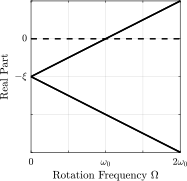
\includegraphics[scale=1]{figs/campbell_diagram_real.png}
\caption{\label{fig:campbell_diagram_real}Campbell Diagram - Real Part}
\end{figure}

\begin{figure}[htbp]
\centering
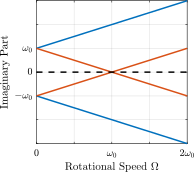
\includegraphics[scale=1]{figs/campbell_diagram_imag.png}
\caption{\label{fig:campbell_diagram_imag}Campbell Diagram - Imaginary Part}
\end{figure}

\section{Simscape Model}
\label{sec:org50f1e50}
In order to validate all the equations of motion, a Simscape model of the same system has been developed.
The dynamics of the system can be identified from the Simscape model and compare with the analytical model.

The rotating speed for the Simscape Model is defined.
\begin{minted}[]{matlab}
  W = 0.1; % Rotation Speed [rad/s]
\end{minted}

\begin{minted}[]{matlab}
  open('rotating_frame.slx');
\end{minted}

The transfer function from \([F_u, F_v]\) to \([d_u, d_v]\) is identified from the Simscape model.

\begin{minted}[]{matlab}
  %% Name of the Simulink File
  mdl = 'rotating_frame';

  %% Input/Output definition
  clear io; io_i = 1;
  io(io_i) = linio([mdl, '/K'], 1, 'openinput');  io_i = io_i + 1;
  io(io_i) = linio([mdl, '/G'], 2, 'openoutput'); io_i = io_i + 1;
\end{minted}

\begin{minted}[]{matlab}
  G = linearize(mdl, io, 0);

  %% Input/Output definition
  G.InputName  = {'Fu', 'Fv'};
  G.OutputName = {'du', 'dv'};
\end{minted}

The same transfer function from \([F_u, F_v]\) to \([d_u, d_v]\) is written down from the analytical model.
\begin{minted}[]{matlab}
  Gth = (1/k)/(((s^2)/(w0^2) + 2*xi*s/w0 + 1 - (W^2)/(w0^2))^2 + (2*W*s/(w0^2))^2) * ...
        [(s^2)/(w0^2) + 2*xi*s/w0 + 1 - (W^2)/(w0^2), 2*W*s/(w0^2) ; ...
         -2*W*s/(w0^2), (s^2)/(w0^2) + 2*xi*s/w0 + 1 - (W^2)/(w0^2)];
\end{minted}

Both transfer functions are compared in Figure \ref{fig:plant_simscape_analytical} and are found to perfectly match.

\begin{figure}[htbp]
\centering
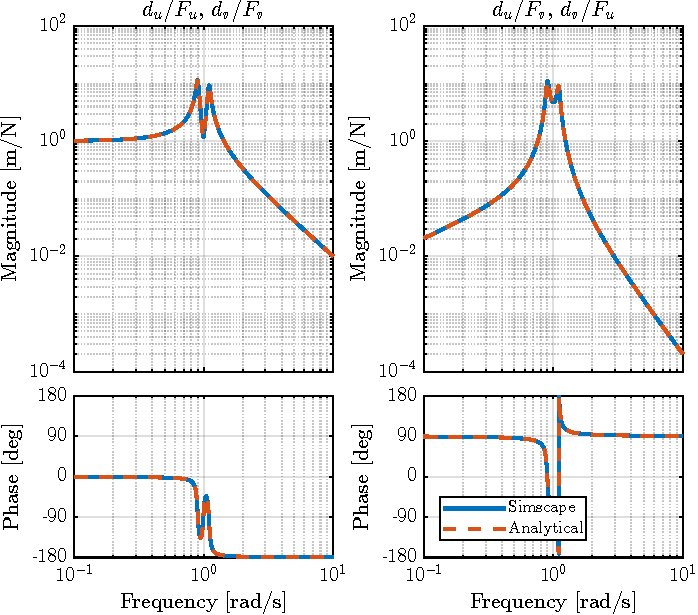
\includegraphics[scale=1]{figs/plant_simscape_analytical.png}
\caption{\label{fig:plant_simscape_analytical}Bode plot of the transfer function from \([F_u, F_v]\) to \([d_u, d_v]\) as identified from the Simscape model and from an analytical model}
\end{figure}

\section{Effect of the rotation speed}
\label{sec:org6d643e3}
The transfer functions from \([F_u, F_v]\) to \([d_u, d_v]\) are identified for the following rotating speeds.
\begin{minted}[]{matlab}
  Ws = [0, 0.2, 0.7, 1.1]*w0; % Rotating Speeds [rad/s]
\end{minted}

\begin{minted}[]{matlab}
  Gs = {zeros(2, 2, length(Ws))};

  for W_i = 1:length(Ws)
      W = Ws(W_i);

      Gs(:, :, W_i) = {(1/k)/(((s^2)/(w0^2) + 2*xi*s/w0 + 1 - (W^2)/(w0^2))^2 + (2*W*s/(w0^2))^2) * ...
                       [(s^2)/(w0^2) + 2*xi*s/w0 + 1 - (W^2)/(w0^2), 2*W*s/(w0^2) ; ...
                        -2*W*s/(w0^2), (s^2)/(w0^2) + 2*xi*s/w0 + 1 - (W^2)/(w0^2)]};
  end
\end{minted}

They are compared in Figures \ref{fig:plant_compare_rotating_speed_direct} and \ref{fig:plant_compare_rotating_speed_coupling}.

\begin{figure}[htbp]
\centering
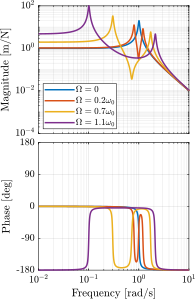
\includegraphics[scale=1]{figs/plant_compare_rotating_speed_direct.png}
\caption{\label{fig:plant_compare_rotating_speed_direct}Comparison of the transfer functions from \([F_u, F_v]\) to \([d_u, d_v]\) for several rotating speed - Direct Terms}
\end{figure}

\begin{figure}[htbp]
\centering
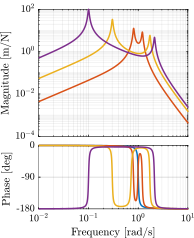
\includegraphics[scale=1]{figs/plant_compare_rotating_speed_coupling.png}
\caption{\label{fig:plant_compare_rotating_speed_coupling}Comparison of the transfer functions from \([F_u, F_v]\) to \([d_u, d_v]\) for several rotating speed - Coupling Terms}
\end{figure}

\chapter{Problem with pure Integral Force Feedback}
\label{sec:org02f3cde}
\label{sec:iff_pure_int}
Force sensors are added in series with the two actuators (Figure \ref{fig:system_iff}).

Two identical controllers \(K_F\) are used to feedback each of the sensed force to its associated actuator.

\begin{figure}[htbp]
\centering
\includegraphics[scale=1]{figs-paper/system_iff.png}
\caption{\label{fig:system_iff}System with added Force Sensor in series with the actuators}
\end{figure}

\section{Plant Parameters}
\label{sec:orgd2d5c32}
Let's define initial values for the model.
\begin{minted}[]{matlab}
  k = 1;    % Actuator Stiffness [N/m]
  c = 0.05; % Actuator Damping [N/(m/s)]
  m = 1;    % Payload mass [kg]
\end{minted}

\begin{minted}[]{matlab}
  xi = c/(2*sqrt(k*m));
  w0 = sqrt(k/m); % [rad/s]
\end{minted}

\section{Equations}
\label{sec:orgad8546b}
The sensed forces are equal to:
\begin{equation}
\begin{bmatrix} f_{u} \\ f_{v} \end{bmatrix} =
\begin{bmatrix}
  1 & 0 \\
  0 & 1
\end{bmatrix}
\begin{bmatrix} F_u \\ F_v \end{bmatrix} - (c s + k)
\begin{bmatrix} d_u \\ d_v \end{bmatrix}
\end{equation}

Which then gives:
\begin{important}
\begin{equation}
\begin{bmatrix} f_{u} \\ f_{v} \end{bmatrix} =
\bm{G}_{f}
\begin{bmatrix} F_u \\ F_v \end{bmatrix}
\end{equation}

\begin{equation}
\begin{bmatrix} f_{u} \\ f_{v} \end{bmatrix} =
\frac{1}{G_{fp}}
\begin{bmatrix}
  G_{fz} & -G_{fc} \\
  G_{fc} &  G_{fz}
\end{bmatrix}
\begin{bmatrix} F_u \\ F_v \end{bmatrix}
\end{equation}

\begin{align}
  G_{fp} &= \left( \frac{s^2}{{\omega_0}^2} + 2 \xi \frac{s}{\omega_0} + 1 - \frac{{\Omega}^2}{{\omega_0}^2} \right)^2 + \left( 2 \frac{\Omega}{\omega_0} \frac{s}{\omega_0} \right)^2 \\
  G_{fz} &= \left( \frac{s^2}{{\omega_0}^2} - \frac{\Omega^2}{{\omega_0}^2} \right) \left( \frac{s^2}{{\omega_0}^2} + 2 \xi \frac{s}{\omega_0} + 1 - \frac{{\Omega}^2}{{\omega_0}^2} \right) + \left( 2 \frac{\Omega}{\omega_0} \frac{s}{\omega_0} \right)^2 \\
  G_{fc} &= \left( 2 \xi \frac{s}{\omega_0} + 1 \right) \left( 2 \frac{\Omega}{\omega_0} \frac{s}{\omega_0} \right)
\end{align}
\end{important}

\section{Comparison of the Analytical Model and the Simscape Model}
\label{sec:org5d37f2f}
The rotation speed is set to \(\Omega = 0.1 \omega_0\).
\begin{minted}[]{matlab}
  W = 0.1*w0; % [rad/s]
\end{minted}

\begin{minted}[]{matlab}
  open('rotating_frame.slx');
\end{minted}

And the transfer function from \([F_u, F_v]\) to \([f_u, f_v]\) is identified using the Simscape model.
\begin{minted}[]{matlab}
  %% Name of the Simulink File
  mdl = 'rotating_frame';

  %% Input/Output definition
  clear io; io_i = 1;
  io(io_i) = linio([mdl, '/K'], 1, 'openinput');  io_i = io_i + 1;
  io(io_i) = linio([mdl, '/G'], 1, 'openoutput'); io_i = io_i + 1;
\end{minted}

\begin{minted}[]{matlab}
  Giff = linearize(mdl, io, 0);

  %% Input/Output definition
  Giff.InputName  = {'Fu', 'Fv'};
  Giff.OutputName = {'fu', 'fv'};
\end{minted}

The same transfer function from \([F_u, F_v]\) to \([f_u, f_v]\) is written down from the analytical model.
\begin{minted}[]{matlab}
  Giff_th = 1/(((s^2)/(w0^2) + 2*xi*s/w0 + 1 - (W^2)/(w0^2))^2 + (2*W*s/(w0^2))^2) * ...
            [(s^2/w0^2 - W^2/w0^2)*((s^2)/(w0^2) + 2*xi*s/w0 + 1 - (W^2)/(w0^2)) + (2*W*s/(w0^2))^2, - (2*xi*s/w0 + 1)*2*W*s/(w0^2) ; ...
             (2*xi*s/w0 + 1)*2*W*s/(w0^2), (s^2/w0^2 - W^2/w0^2)*((s^2)/(w0^2) + 2*xi*s/w0 + 1 - (W^2)/(w0^2))+ (2*W*s/(w0^2))^2];
\end{minted}

The two are compared in Figure \ref{fig:plant_iff_comp_simscape_analytical} and found to perfectly match.
\begin{figure}[htbp]
\centering
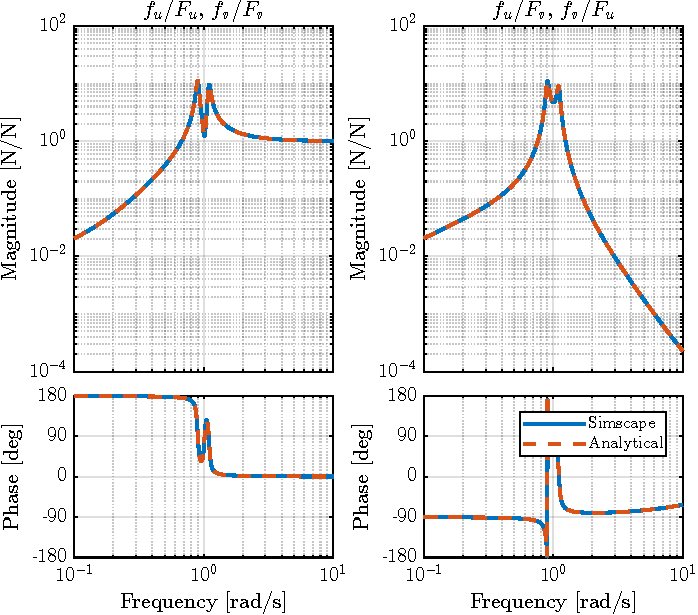
\includegraphics[scale=1]{figs/plant_iff_comp_simscape_analytical.png}
\caption{\label{fig:plant_iff_comp_simscape_analytical}Comparison of the transfer functions from \([F_u, F_v]\) to \([f_u, f_v]\) between the Simscape model and the analytical one}
\end{figure}

\section{Effect of the rotation speed}
\label{sec:org17fee48}
The transfer functions from \([F_u, F_v]\) to \([f_u, f_v]\) are identified for the following rotating speeds.
\begin{minted}[]{matlab}
  Ws = [0, 0.2, 0.7]*w0; % Rotating Speeds [rad/s]
\end{minted}

\begin{minted}[]{matlab}
  Gsiff = {zeros(2, 2, length(Ws))};

  for W_i = 1:length(Ws)
      W = Ws(W_i);

      Gsiff(:, :, W_i) = {1/(((s^2)/(w0^2) + 2*xi*s/w0 + 1 - (W^2)/(w0^2))^2 + (2*W*s/(w0^2))^2) * ...
                        [(s^2/w0^2 - W^2/w0^2)*((s^2)/(w0^2) + 2*xi*s/w0 + 1 - (W^2)/(w0^2)) + (2*W*s/(w0^2))^2, - (2*xi*s/w0 + 1)*2*W*s/(w0^2) ; ...
                         (2*xi*s/w0 + 1)*2*W*s/(w0^2), (s^2/w0^2 - W^2/w0^2)*((s^2)/(w0^2) + 2*xi*s/w0 + 1 - (W^2)/(w0^2))+ (2*W*s/(w0^2))^2]};
  end
\end{minted}

The obtained transfer functions are shown in Figure \ref{fig:plant_iff_compare_rotating_speed}.
\begin{figure}[htbp]
\centering
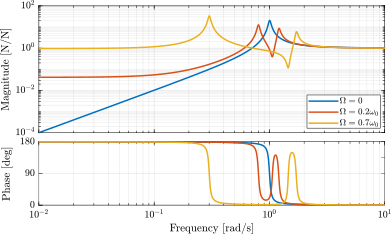
\includegraphics[scale=1]{figs/plant_iff_compare_rotating_speed.png}
\caption{\label{fig:plant_iff_compare_rotating_speed}Comparison of the transfer functions from \([F_u, F_v]\) to \([f_u, f_v]\) for several rotating speed}
\end{figure}

\section{Decentralized Integral Force Feedback}
\label{sec:org2d5427a}
The decentralized IFF controller consists of pure integrators:
\begin{equation}
  \bm{K}_{\text{IFF}}(s) = \frac{g}{s} \begin{bmatrix}
    1 & 0 \\
    0 & 1
  \end{bmatrix}
\end{equation}

The Root Locus (evolution of the poles of the closed loop system in the complex plane as a function of \(g\)) is shown in Figure \ref{fig:root_locus_pure_iff}.
It is shown that for non-null rotating speed, one pole is bound to the right-half plane, and thus the closed loop system is unstable.

\begin{figure}[htbp]
\centering
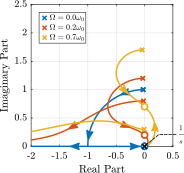
\includegraphics[scale=1]{figs/root_locus_pure_iff.png}
\caption{\label{fig:root_locus_pure_iff}Root Locus for the Decentralized Integral Force Feedback controller. Several rotating speed are shown.}
\end{figure}

\chapter{Integral Force Feedback with an High Pass Filter}
\label{sec:orgf9854e9}
\label{sec:iff_pseudo_int}

\section{Plant Parameters}
\label{sec:org11b9a15}
Let's define initial values for the model.
\begin{minted}[]{matlab}
  k = 1;    % Actuator Stiffness [N/m]
  c = 0.05; % Actuator Damping [N/(m/s)]
  m = 1;    % Payload mass [kg]
\end{minted}

\begin{minted}[]{matlab}
  xi = c/(2*sqrt(k*m));
  w0 = sqrt(k/m); % [rad/s]
\end{minted}

\section{Modified Integral Force Feedback Controller}
\label{sec:orgf920a8a}
Let's modify the initial Integral Force Feedback Controller ; instead of using pure integrators, pseudo integrators (i.e. low pass filters) are used:
\begin{equation}
  K_{\text{IFF}}(s) = g\frac{1}{\omega_i + s} \begin{bmatrix}
  1 & 0 \\
  0 & 1
\end{bmatrix}
\end{equation}
where \(\omega_i\) characterize down to which frequency the signal is integrated.

Let's arbitrary choose the following control parameters:
\begin{minted}[]{matlab}
  g = 2;
  wi = 0.1*w0;
\end{minted}

And the following rotating speed.
\begin{minted}[]{matlab}
  Giff = 1/(((s^2)/(w0^2) + 2*xi*s/w0 + 1 - (W^2)/(w0^2))^2 + (2*W*s/(w0^2))^2) * ...
          [(s^2/w0^2 - W^2/w0^2)*((s^2)/(w0^2) + 2*xi*s/w0 + 1 - (W^2)/(w0^2)) + (2*W*s/(w0^2))^2, - (2*xi*s/w0 + 1)*2*W*s/(w0^2) ; ...
           (2*xi*s/w0 + 1)*2*W*s/(w0^2), (s^2/w0^2 - W^2/w0^2)*((s^2)/(w0^2) + 2*xi*s/w0 + 1 - (W^2)/(w0^2))+ (2*W*s/(w0^2))^2];
\end{minted}

The obtained Loop Gain is shown in Figure \ref{fig:loop_gain_modified_iff}.
\begin{figure}[htbp]
\centering
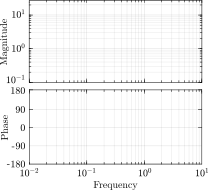
\includegraphics[scale=1]{figs/loop_gain_modified_iff.png}
\caption{\label{fig:loop_gain_modified_iff}Loop Gain for the modified IFF controller}
\end{figure}

\section{Root Locus}
\label{sec:org911f45b}
As shown in the Root Locus plot (Figure \ref{fig:root_locus_modified_iff}), for some value of the gain, the system remains stable.

\begin{figure}[htbp]
\centering
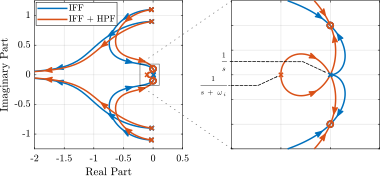
\includegraphics[scale=1]{figs/root_locus_modified_iff.png}
\caption{\label{fig:root_locus_modified_iff}Root Locus for the modified IFF controller}
\end{figure}

\begin{figure}[htbp]
\centering
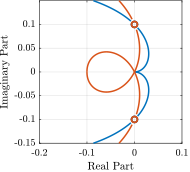
\includegraphics[scale=1]{figs/root_locus_modified_iff_zoom.png}
\caption{\label{fig:root_locus_modified_iff_zoom}Root Locus for the modified IFF controller - Zoom}
\end{figure}

\section{What is the optimal \(\omega_i\) and \(g\)?}
\label{sec:org028e747}
In order to visualize the effect of \(\omega_i\) on the attainable damping, the Root Locus is displayed in Figure \ref{fig:root_locus_wi_modified_iff} for the following \(\omega_i\):
\begin{minted}[]{matlab}
  wis = [0.01, 0.1, 0.5, 1]*w0; % [rad/s]
\end{minted}

\begin{figure}[htbp]
\centering
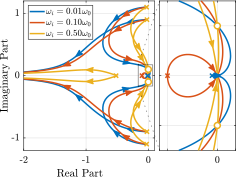
\includegraphics[scale=1]{figs/root_locus_wi_modified_iff.png}
\caption{\label{fig:root_locus_wi_modified_iff}Root Locus for the modified IFF controller (zoomed plot on the left)}
\end{figure}

\begin{figure}[htbp]
\centering
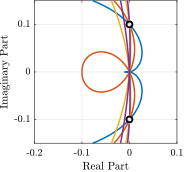
\includegraphics[scale=1]{figs/root_locus_wi_modified_iff_zoom.png}
\caption{\label{fig:root_locus_wi_modified_iff_zoom}Root Locus for the modified IFF controller (zoomed plot on the left)}
\end{figure}

For the controller
\begin{equation}
  K_{\text{IFF}}(s) = g\frac{1}{\omega_i + s} \begin{bmatrix}
  1 & 0 \\
  0 & 1
\end{bmatrix}
\end{equation}
The gain at which the system becomes unstable is
\begin{equation}
  g_\text{max} = \omega_i \left( \frac{{\omega_0}^2}{\Omega^2} - 1 \right) \label{eq:iff_gmax}
\end{equation}

While it seems that small \(\omega_i\) do allow more damping to be added to the system (Figure \ref{fig:root_locus_wi_modified_iff}), the control gains may be limited to small values due to \eqref{eq:iff_gmax} thus reducing the attainable damping.

There must be an optimum for \(\omega_i\).
To find the optimum, the gain that maximize the simultaneous damping of the mode is identified for a wide range of \(\omega_i\) (Figure \ref{fig:mod_iff_damping_wi}).

\begin{minted}[]{matlab}
  wis = logspace(-2, 1, 100)*w0; % [rad/s]

  opt_xi = zeros(1, length(wis)); % Optimal simultaneous damping
  opt_gain = zeros(1, length(wis)); % Corresponding optimal gain

  for wi_i = 1:length(wis)
      wi = wis(wi_i);
      Kiff = 1/(s + wi)*eye(2);

      fun = @(g)computeSimultaneousDamping(g, Giff, Kiff);

      [g_opt, xi_opt] = fminsearch(fun, 0.5*wi*((w0/W)^2 - 1));
      opt_xi(wi_i) = 1/xi_opt;
      opt_gain(wi_i) = g_opt;
  end
\end{minted}

\begin{figure}[htbp]
\centering
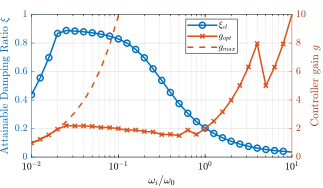
\includegraphics[scale=1]{figs/mod_iff_damping_wi.png}
\caption{\label{fig:mod_iff_damping_wi}Simultaneous attainable damping of the closed loop poles as a function of \(\omega_i\)}
\end{figure}

\chapter{IFF with a stiffness in parallel with the force sensor}
\label{sec:orgc5ba04a}
\label{sec:iff_parallel_stiffness}

\section{Schematic}
\label{sec:orgc647af5}
In this section additional springs in parallel with the force sensors are added to counteract the negative stiffness induced by the rotation.

\begin{figure}[htbp]
\centering
\includegraphics[scale=1]{figs-paper/system_parallel_springs.png}
\caption{\label{fig:system_parallel_springs}Studied system with additional springs in parallel with the actuators and force sensors}
\end{figure}

In order to keep the overall stiffness \(k = k_a + k_p\) constant, a scalar parameter \(\alpha\) (\(0 \le \alpha < 1\)) is defined to describe the fraction of the total stiffness in parallel with the actuator and force sensor
\begin{equation}
  k_p = \alpha k, \quad k_a = (1 - \alpha) k
\end{equation}

\section{Equations}
\label{sec:org0de17db}
\begin{important}
\begin{equation}
\begin{bmatrix} f_u \\ f_v \end{bmatrix} =
\bm{G}_k
\begin{bmatrix} F_u \\ F_v \end{bmatrix}
\end{equation}

\begin{equation}
\begin{bmatrix} f_u \\ f_v \end{bmatrix} =
\frac{1}{G_{kp}}
\begin{bmatrix}
   G_{kz} & -G_{kc} \\
   G_{kc} &  G_{kz}
\end{bmatrix}
\begin{bmatrix} F_u \\ F_v \end{bmatrix}
\end{equation}
With:
\begin{align}
  G_{kp} &= \left( \frac{s^2}{{\omega_0}^2} + 2\xi \frac{s}{{\omega_0}^2} + 1 - \frac{\Omega^2}{{\omega_0}^2} \right)^2 + \left( 2 \frac{\Omega}{\omega_0}\frac{s}{\omega_0} \right)^2 \\
  G_{kz} &= \left( \frac{s^2}{{\omega_0}^2} - \frac{\Omega^2}{{\omega_0}^2} + \alpha \right) \left( \frac{s^2}{{\omega_0}^2} + 2\xi \frac{s}{{\omega_0}^2} + 1 - \frac{\Omega^2}{{\omega_0}^2} \right) + \left( 2 \frac{\Omega}{\omega_0}\frac{s}{\omega_0} \right)^2 \\
  G_{kc} &= \left( 2 \xi \frac{s}{\omega_0} + 1 - \alpha \right) \left( 2 \frac{\Omega}{\omega_0}\frac{s}{\omega_0} \right)
\end{align}
\end{important}

If we compare \(G_{kz}\) and \(G_{fz}\), we see that the spring in parallel adds a term \(\alpha\).
In order to have two complex conjugate zeros (instead of real zeros):
\begin{equation}
  \alpha > \frac{\Omega^2}{{\omega_0}^2} \quad \Leftrightarrow \quad k_p > m \Omega^2
\end{equation}

\section{Plant Parameters}
\label{sec:orga1e1958}
Let's define initial values for the model.
\begin{minted}[]{matlab}
  k = 1;    % Actuator Stiffness [N/m]
  c = 0.05; % Actuator Damping [N/(m/s)]
  m = 1;    % Payload mass [kg]
\end{minted}

\begin{minted}[]{matlab}
  xi = c/(2*sqrt(k*m));
  w0 = sqrt(k/m); % [rad/s]
\end{minted}

\section{Comparison of the Analytical Model and the Simscape Model}
\label{sec:orgbea84d1}
The same transfer function from \([F_u, F_v]\) to \([f_u, f_v]\) is written down from the analytical model.
\begin{minted}[]{matlab}
  W = 0.1*w0; % [rad/s]

  kp = 1.5*m*W^2;
  cp = 0;
\end{minted}

\begin{minted}[]{matlab}
  open('rotating_frame.slx');
\end{minted}

\begin{minted}[]{matlab}
  %% Name of the Simulink File
  mdl = 'rotating_frame';

  %% Input/Output definition
  clear io; io_i = 1;
  io(io_i) = linio([mdl, '/K'], 1, 'openinput');  io_i = io_i + 1;
  io(io_i) = linio([mdl, '/G'], 1, 'openoutput'); io_i = io_i + 1;

  Giff = linearize(mdl, io, 0);

  %% Input/Output definition
  Giff.InputName  = {'Fu', 'Fv'};
  Giff.OutputName = {'fu', 'fv'};
\end{minted}

\begin{minted}[]{matlab}
  w0p = sqrt((k + kp)/m);
  xip = c/(2*sqrt((k+kp)*m));

  Giff_th = 1/( (s^2/w0p^2 + 2*xip*s/w0p + 1 - W^2/w0p^2)^2 + (2*(s/w0p)*(W/w0p))^2 ) * [ ...
                     (s^2/w0p^2 + kp/(k + kp) - W^2/w0p^2)*(s^2/w0p^2 + 2*xip*s/w0p + 1 - W^2/w0p^2) + (2*(s/w0p)*(W/w0p))^2, -(2*xip*s/w0p + k/(k + kp))*(2*(s/w0p)*(W/w0p));
                     (2*xip*s/w0p + k/(k + kp))*(2*(s/w0p)*(W/w0p)), (s^2/w0p^2 + kp/(k + kp) - W^2/w0p^2)*(s^2/w0p^2 + 2*xip*s/w0p + 1 - W^2/w0p^2) + (2*(s/w0p)*(W/w0p))^2 ];
  Giff_th.InputName  = {'Fu', 'Fv'};
  Giff_th.OutputName = {'fu', 'fv'};
\end{minted}

\begin{figure}[htbp]
\centering
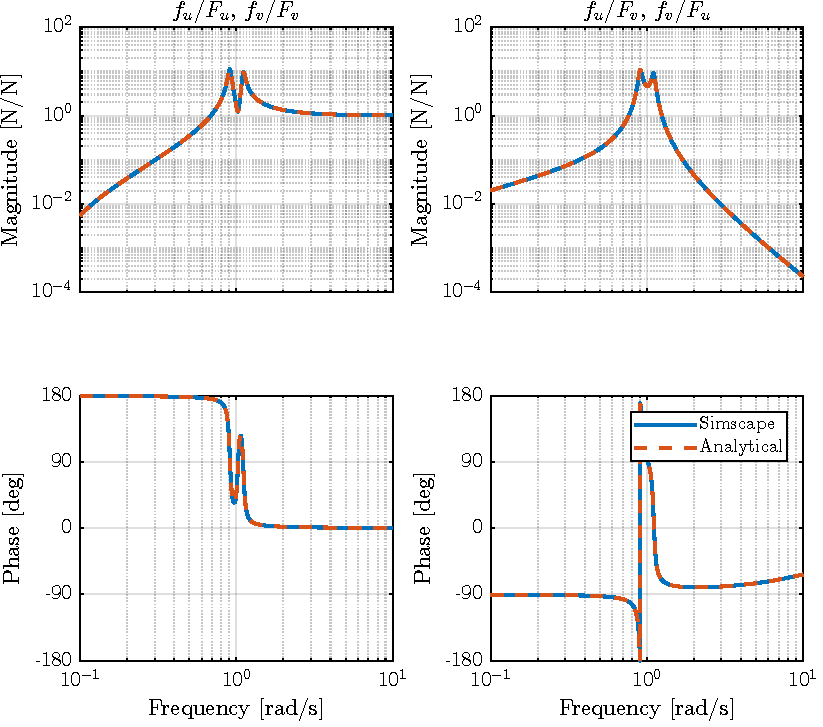
\includegraphics[scale=1]{figs/plant_iff_kp_comp_simscape_analytical.png}
\caption{\label{fig:plant_iff_kp_comp_simscape_analytical}Comparison of the transfer functions from \([F_u, F_v]\) to \([f_u, f_v]\) between the Simscape model and the analytical one}
\end{figure}

\section{Effect of the parallel stiffness on the IFF plant}
\label{sec:orge9068cb}
The rotation speed is set to \(\Omega = 0.1 \omega_0\).
\begin{minted}[]{matlab}
  W = 0.1*w0; % [rad/s]
\end{minted}

And the IFF plant (transfer function from \([F_u, F_v]\) to \([f_u, f_v]\)) is identified in three different cases:
\begin{itemize}
\item without parallel stiffness
\item with a small parallel stiffness \(k_p < m \Omega^2\)
\item with a large parallel stiffness \(k_p > m \Omega^2\)
\end{itemize}

The results are shown in Figure \ref{fig:plant_iff_kp}.

One can see that for \(k_p > m \Omega^2\), the systems shows alternating complex conjugate poles and zeros.

\begin{minted}[]{matlab}
  kp = 0;

  w0p = sqrt((k + kp)/m);
  xip = c/(2*sqrt((k+kp)*m));

  Giff = 1/( (s^2/w0p^2 + 2*xip*s/w0p + 1 - W^2/w0p^2)^2 + (2*(s/w0p)*(W/w0p))^2 ) * [ ...
      (s^2/w0p^2 + kp/(k + kp) - W^2/w0p^2)*(s^2/w0p^2 + 2*xip*s/w0p + 1 - W^2/w0p^2) + (2*(s/w0p)*(W/w0p))^2, -(2*xip*s/w0p + k/(k + kp))*(2*(s/w0p)*(W/w0p));
      (2*xip*s/w0p + k/(k + kp))*(2*(s/w0p)*(W/w0p)), (s^2/w0p^2 + kp/(k + kp) - W^2/w0p^2)*(s^2/w0p^2 + 2*xip*s/w0p + 1 - W^2/w0p^2) + (2*(s/w0p)*(W/w0p))^2];
\end{minted}

\begin{minted}[]{matlab}
  kp = 0.5*m*W^2;
  k = 1 - kp;

  w0p = sqrt((k + kp)/m);
  xip = c/(2*sqrt((k+kp)*m));

  Giff_s = 1/( (s^2/w0p^2 + 2*xip*s/w0p + 1 - W^2/w0p^2)^2 + (2*(s/w0p)*(W/w0p))^2 ) * [ ...
      (s^2/w0p^2 + kp/(k + kp) - W^2/w0p^2)*(s^2/w0p^2 + 2*xip*s/w0p + 1 - W^2/w0p^2) + (2*(s/w0p)*(W/w0p))^2, -(2*xip*s/w0p + k/(k + kp))*(2*(s/w0p)*(W/w0p));
      (2*xip*s/w0p + k/(k + kp))*(2*(s/w0p)*(W/w0p)), (s^2/w0p^2 + kp/(k + kp) - W^2/w0p^2)*(s^2/w0p^2 + 2*xip*s/w0p + 1 - W^2/w0p^2) + (2*(s/w0p)*(W/w0p))^2];
\end{minted}

\begin{minted}[]{matlab}
  kp = 1.5*m*W^2;
  k = 1 - kp;

  w0p = sqrt((k + kp)/m);
  xip = c/(2*sqrt((k+kp)*m));

  Giff_l = 1/( (s^2/w0p^2 + 2*xip*s/w0p + 1 - W^2/w0p^2)^2 + (2*(s/w0p)*(W/w0p))^2 ) * [ ...
      (s^2/w0p^2 + kp/(k + kp) - W^2/w0p^2)*(s^2/w0p^2 + 2*xip*s/w0p + 1 - W^2/w0p^2) + (2*(s/w0p)*(W/w0p))^2, -(2*xip*s/w0p + k/(k + kp))*(2*(s/w0p)*(W/w0p));
      (2*xip*s/w0p + k/(k + kp))*(2*(s/w0p)*(W/w0p)), (s^2/w0p^2 + kp/(k + kp) - W^2/w0p^2)*(s^2/w0p^2 + 2*xip*s/w0p + 1 - W^2/w0p^2) + (2*(s/w0p)*(W/w0p))^2];
\end{minted}

\begin{figure}[htbp]
\centering
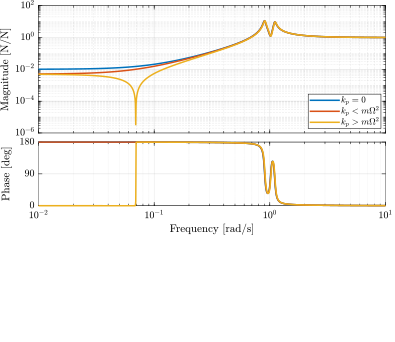
\includegraphics[scale=1]{figs/plant_iff_kp.png}
\caption{\label{fig:plant_iff_kp}Transfer function from \([F_u, F_v]\) to \([f_u, f_v]\) for \(k_p = 0\), \(k_p < m \Omega^2\) and \(k_p > m \Omega^2\)}
\end{figure}

\section{IFF when adding a spring in parallel}
\label{sec:org9f1e3df}
In Figure \ref{fig:root_locus_iff_kp} is displayed the Root Locus in the three considered cases with
\begin{equation}
  K_{\text{IFF}} = \frac{g}{s} \begin{bmatrix}
  1 & 0 \\
  0 & 1
\end{bmatrix}
\end{equation}

One can see that for \(k_p > m \Omega^2\), the root locus stays in the left half of the complex plane and thus the control system is unconditionally stable.

Thus, decentralized IFF controller with pure integrators can be used if:
\begin{equation}
  k_{p} > m \Omega^2
\end{equation}

\begin{figure}[htbp]
\centering
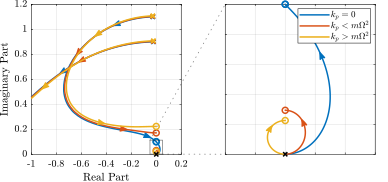
\includegraphics[scale=1]{figs/root_locus_iff_kp.png}
\caption{\label{fig:root_locus_iff_kp}Root Locus}
\end{figure}

\begin{figure}[htbp]
\centering
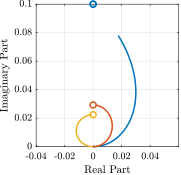
\includegraphics[scale=1]{figs/root_locus_iff_kp_zoom.png}
\caption{\label{fig:root_locus_iff_kp_zoom}Root Locus}
\end{figure}

\section{Effect of \(k_p\) on the attainable damping}
\label{sec:orgcb7905c}
However, having large values of \(k_p\) may decrease the attainable damping.

To study the second point, Root Locus plots for the following values of \(k_p\) are shown in Figure \ref{fig:root_locus_iff_kps}.
\begin{minted}[]{matlab}
  kps = [2, 20, 40]*m*W^2;
\end{minted}

It is shown that large values of \(k_p\) decreases the attainable damping.
\begin{figure}[htbp]
\centering
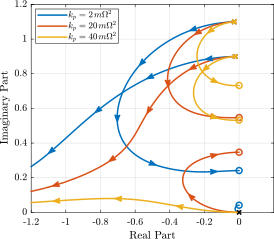
\includegraphics[scale=1]{figs/root_locus_iff_kps.png}
\caption{\label{fig:root_locus_iff_kps}Root Locus plot}
\end{figure}

\begin{minted}[]{matlab}
  alphas = logspace(-2, 0, 100);

  opt_xi = zeros(1, length(alphas)); % Optimal simultaneous damping
  opt_gain = zeros(1, length(alphas)); % Corresponding optimal gain

  Kiff = 1/s*eye(2);

  for alpha_i = 1:length(alphas)
      kp = alphas(alpha_i);
      k = 1 - alphas(alpha_i);

      w0p = sqrt((k + kp)/m);
      xip = c/(2*sqrt((k+kp)*m));

      Giff = 1/( (s^2/w0p^2 + 2*xip*s/w0p + 1 - W^2/w0p^2)^2 + (2*(s/w0p)*(W/w0p))^2 ) * [ ...
          (s^2/w0p^2 + kp/(k + kp) - W^2/w0p^2)*(s^2/w0p^2 + 2*xip*s/w0p + 1 - W^2/w0p^2) + (2*(s/w0p)*(W/w0p))^2, -(2*xip*s/w0p + k/(k + kp))*(2*(s/w0p)*(W/w0p));
          (2*xip*s/w0p + k/(k + kp))*(2*(s/w0p)*(W/w0p)), (s^2/w0p^2 + kp/(k + kp) - W^2/w0p^2)*(s^2/w0p^2 + 2*xip*s/w0p + 1 - W^2/w0p^2) + (2*(s/w0p)*(W/w0p))^2];

      fun = @(g)computeSimultaneousDamping(g, Giff, Kiff);

      [g_opt, xi_opt] = fminsearch(fun, 2);
      opt_xi(alpha_i) = 1/xi_opt;
      opt_gain(alpha_i) = g_opt;
  end
\end{minted}

\begin{figure}[htbp]
\centering
\includegraphics[scale=1]{figs/opt_damp_alpha.png}
\caption{\label{fig:opt_damp_alpha}Attainable damping ratio and corresponding controller gain for different parameter \(\alpha\)}
\end{figure}

\chapter{Comparison}
\label{sec:org4714bd6}
\label{sec:comparison}
Two modifications to adapt the IFF control strategy to rotating platforms have been proposed.
These two methods are now compared in terms of added damping, closed-loop compliance and transmissibility.

\section{Plant Parameters}
\label{sec:org90a54af}
Let's define initial values for the model.
\begin{minted}[]{matlab}
  k = 1;    % Actuator Stiffness [N/m]
  c = 0.05; % Actuator Damping [N/(m/s)]
  m = 1;    % Payload mass [kg]
\end{minted}

\begin{minted}[]{matlab}
  xi = c/(2*sqrt(k*m));
  w0 = sqrt(k/m); % [rad/s]
\end{minted}

The rotating speed is set to \(\Omega = 0.1 \omega_0\).
\begin{minted}[]{matlab}
  W = 0.1*w0;
\end{minted}

\section{Root Locus}
\label{sec:orgf922463}
IFF with High Pass Filter
\begin{minted}[]{matlab}
  wi = 0.1*w0; % [rad/s]

  Giff = 1/(((s^2)/(w0^2) + 2*xi*s/w0 + 1 - (W^2)/(w0^2))^2 + (2*W*s/(w0^2))^2) * ...
          [(s^2/w0^2 - W^2/w0^2)*((s^2)/(w0^2) + 2*xi*s/w0 + 1 - (W^2)/(w0^2)) + (2*W*s/(w0^2))^2, - (2*xi*s/w0 + 1)*2*W*s/(w0^2) ; ...
           (2*xi*s/w0 + 1)*2*W*s/(w0^2), (s^2/w0^2 - W^2/w0^2)*((s^2)/(w0^2) + 2*xi*s/w0 + 1 - (W^2)/(w0^2))+ (2*W*s/(w0^2))^2];
\end{minted}

IFF With parallel Stiffness
\begin{minted}[]{matlab}
  kp = 5*m*W^2;
  k = k - kp;

  w0p = sqrt((k + kp)/m);
  xip = c/(2*sqrt((k+kp)*m));

  Giff_kp = 1/( (s^2/w0p^2 + 2*xip*s/w0p + 1 - W^2/w0p^2)^2 + (2*(s/w0p)*(W/w0p))^2 ) * [ ...
                     (s^2/w0p^2 + kp/(k + kp) - W^2/w0p^2)*(s^2/w0p^2 + 2*xip*s/w0p + 1 - W^2/w0p^2) + (2*(s/w0p)*(W/w0p))^2, -(2*xip*s/w0p + k/(k + kp))*(2*(s/w0p)*(W/w0p));
                     (2*xip*s/w0p + k/(k + kp))*(2*(s/w0p)*(W/w0p)), (s^2/w0p^2 + kp/(k + kp) - W^2/w0p^2)*(s^2/w0p^2 + 2*xip*s/w0p + 1 - W^2/w0p^2) + (2*(s/w0p)*(W/w0p))^2 ];

  k = k + kp;
\end{minted}

\begin{figure}[htbp]
\centering
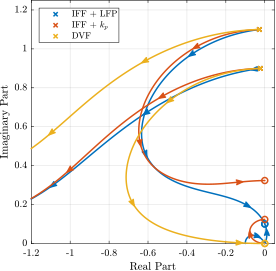
\includegraphics[scale=1]{figs/comp_root_locus.png}
\caption{\label{fig:comp_root_locus}Root Locus plot - Comparison of IFF with additional high pass filter, IFF with additional parallel stiffness}
\end{figure}

\section{Controllers - Optimal Gains}
\label{sec:org1889cfc}
In order to compare to three considered Active Damping techniques, gains that yield maximum damping of all the modes are computed for each case.

The obtained damping ratio and control are shown below.

\begin{center}
\begin{tabular}{lrr}
 & Obtained \(\xi\) & Control Gain\\
\hline
Modified IFF & 0.83 & 1.99\\
IFF with \(k_p\) & 0.83 & 2.02\\
\end{tabular}
\end{center}

\section{Passive Damping - Critical Damping}
\label{sec:org81b0306}
\begin{equation}
  \xi = \frac{c}{2 \sqrt{km}}
\end{equation}

Critical Damping corresponds to to \(\xi = 1\), and thus:
\begin{equation}
  c_{\text{crit}} = 2 \sqrt{km}
\end{equation}

\begin{minted}[]{matlab}
  c_opt = 2*sqrt(k*m);
\end{minted}

\section{Transmissibility And Compliance}
\label{sec:orge56633c}
\label{sec:comp_transmissibilty}

\begin{minted}[]{matlab}
  open('rotating_frame.slx');
\end{minted}

\begin{minted}[]{matlab}
  %% Name of the Simulink File
  mdl = 'rotating_frame';

  %% Input/Output definition
  clear io; io_i = 1;
  io(io_i) = linio([mdl, '/dw'], 1, 'input');  io_i = io_i + 1;
  io(io_i) = linio([mdl, '/fd'], 1, 'input');  io_i = io_i + 1;
  io(io_i) = linio([mdl, '/Meas'], 1, 'output');  io_i = io_i + 1;
\end{minted}
\begin{minted}[]{matlab}
  G_ol = linearize(mdl, io, 0);

  %% Input/Output definition
  G_ol.InputName  = {'Dwx', 'Dwy', 'Fdx', 'Fdy'};
  G_ol.OutputName = {'Dx', 'Dy'};
\end{minted}

\subsection{Passive Damping}
\label{sec:orgc0de759}
\begin{minted}[]{matlab}
  kp = 0;
  cp = 0;
\end{minted}

\begin{minted}[]{matlab}
  c_old = c;
  c = c_opt;
\end{minted}

\begin{minted}[]{matlab}
  G_pas = linearize(mdl, io, 0);

  %% Input/Output definition
  G_pas.InputName  = {'Dwx', 'Dwy', 'Fdx', 'Fdy'};
  G_pas.OutputName = {'Dx', 'Dy'};
\end{minted}

\begin{minted}[]{matlab}
  c = c_old;
\end{minted}

\begin{minted}[]{matlab}
  Kiff = opt_gain_iff/(wi + s)*tf(eye(2));
\end{minted}

\begin{minted}[]{matlab}
  G_iff = linearize(mdl, io, 0);

  %% Input/Output definition
  G_iff.InputName  = {'Dwx', 'Dwy', 'Fdx', 'Fdy'};
  G_iff.OutputName = {'Dx', 'Dy'};
\end{minted}

\begin{minted}[]{matlab}
  kp = 5*m*W^2;
  cp = 0.01;
\end{minted}

\begin{minted}[]{matlab}
  Kiff = opt_gain_kp/s*tf(eye(2));
\end{minted}

\begin{minted}[]{matlab}
  G_kp = linearize(mdl, io, 0);

  %% Input/Output definition
  G_kp.InputName  = {'Dwx', 'Dwy', 'Fdx', 'Fdy'};
  G_kp.OutputName = {'Dx', 'Dy'};
\end{minted}

\begin{figure}[htbp]
\centering
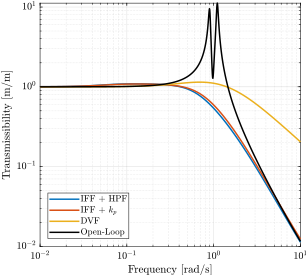
\includegraphics[scale=1]{figs/comp_transmissibility.png}
\caption{\label{fig:comp_transmissibility}Comparison of the transmissibility}
\end{figure}

\begin{figure}[htbp]
\centering
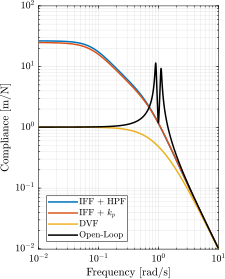
\includegraphics[scale=1]{figs/comp_compliance.png}
\caption{\label{fig:comp_compliance}Comparison of the obtained Compliance}
\end{figure}

\chapter{Notations}
\label{sec:org61801fb}
\label{sec:notations}

\begin{center}
\begin{tabular}{llll}
 & Mathematical Notation & Matlab & Unit\\
\hline
Actuator Stiffness & \(k\) & \texttt{k} & N/m\\
Actuator Damping & \(c\) & \texttt{c} & N/(m/s)\\
Payload Mass & \(m\) & \texttt{m} & kg\\
Damping Ratio & \(\xi = \frac{c}{2\sqrt{km}}\) & \texttt{xi} & \\
Actuator Force & \(\bm{F}, F_u, F_v\) & \texttt{F} \texttt{Fu} \texttt{Fv} & N\\
Force Sensor signal & \(\bm{f}, f_u, f_v\) & \texttt{f} \texttt{fu} \texttt{fv} & N\\
Relative Displacement & \(\bm{d}, d_u, d_v\) & \texttt{d} \texttt{du} \texttt{dv} & m\\
Resonance freq. when \(\Omega = 0\) & \(\omega_0\) & \texttt{w0} & rad/s\\
Rotation Speed & \(\Omega = \dot{\theta}\) & \texttt{W} & rad/s\\
Low Pass Filter corner frequency & \(\omega_i\) & \texttt{wi} & rad/s\\
\end{tabular}
\end{center}

\begin{center}
\begin{tabular}{llll}
 & Mathematical Notation & Matlab & Unit\\
\hline
Laplace variable & \(s\) & \texttt{s} & \\
Complex number & \(j\) & \texttt{j} & \\
Frequency & \(\omega\) & \texttt{w} & [rad/s]\\
\end{tabular}
\end{center}

\printbibliography

\bibliography{ref}
\end{document}
